\begin{figure}[h]
    \centering

    \begin{subfigure}[b]{0.45\textwidth}
        \centering
        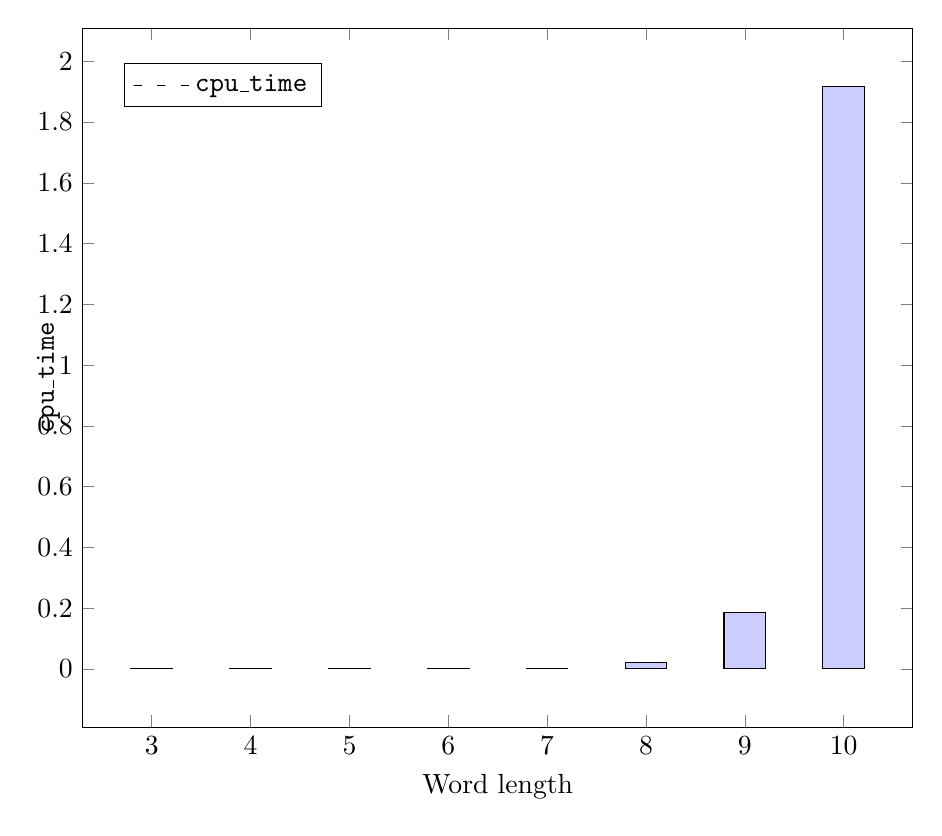
\begin{tikzpicture}
            \begin{axis}[
                xlabel=Word length,
                ylabel=\texttt{cpu\_time},
                ylabel style={yshift=-15pt},
                xtick=data,
                width=\linewidth,
                legend style={at={(0.05,0.95)},anchor=north west},
                ]
            \addplot[ybar, bar width=15pt, fill=blue!20]
                coordinates {
                    (3, 5.6425730387369794e-06)(4, 1.9073486328125e-05)(5, 8.714900297277113e-05)(6, 0.0004047552744547526)(7, 0.0025780797004699707)(8, 0.02060066952424891)(9, 0.18696789308027786)(10, 1.9171473185221355)
                    };
            \legend{ \texttt{cpu\_time} } 
            \end{axis}
        \end{tikzpicture}
    \end{subfigure}
    % \hfill
    \begin{subfigure}[b]{0.45\textwidth}
        \centering
        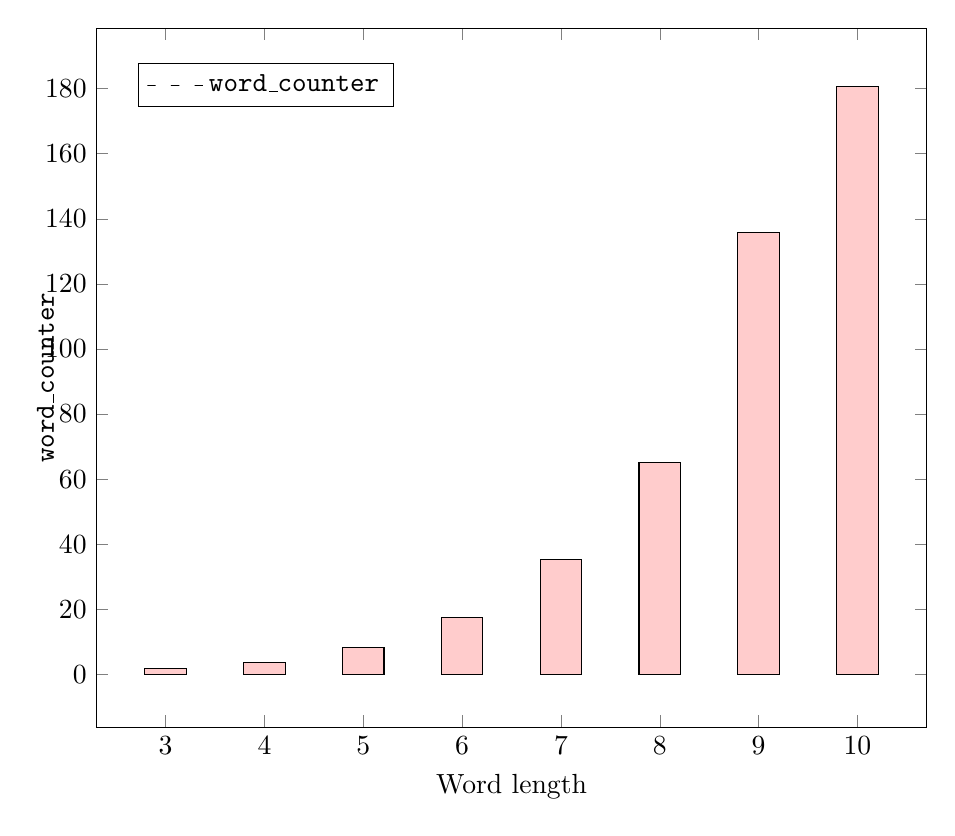
\begin{tikzpicture}
            \begin{axis}[
                xlabel=Word length,
                width=\linewidth,
                ylabel=\texttt{word\_counter},
                ylabel style={yshift=-10pt},
                xtick=data,
                legend style={at={(0.05,0.95)},anchor=north west}
                ]
            \addplot[ybar, bar width=15pt, fill=red!20]
                coordinates {
                    (3, 1.6666666666666667)(4, 3.7)(5, 8.294117647058824)(6, 17.428571428571427)(7, 35.25)(8, 65.23529411764706)(9, 135.9090909090909)(10, 180.66666666666666)
                    };
            \legend{ \texttt{word\_counter} } 
            \end{axis}
        \end{tikzpicture}
    \end{subfigure}
    \caption{Performances testing through process}
\end{figure}